
\appendix

\section{Appendiks - Installasjon av Linux}\label{4-appendix}

Det er mulig å installere Linux på egen maskin i tillegg til å bruke maskinene på Sanntidsalen. Dette gjøres enten ved å slette operativsystemet man har nå for så å installere Linux, eller gjennom en ordning kalt \textit{dual booting}. Sistenevnte er spesielt populært og betyr ganske greit at man har to eller flere operativsystemer installert på en datamaskin, så velger man hvilket operativsystem man vil \textit{boote} inn ved oppstart.

Installasjonsprosessen er litt forskjellig fra maskin til maskin, og Linux-variant, men her er en generell beskrivelse av installasjons-prosessen.

\subsection{Last ned operativsystemet}\label{app:linux-last}

Det første man trenger er et \textit{image} av operativsystemet man vil installere. Om dette er første gang man er borti Linux før, er Ubuntu anbefalt. Fra \href{https://ubuntu.com/download}{https://ubuntu\newline.com/download} kan man laste ned nyeste LTS-utgave (\textbf{L}ong \textbf{T}erm \textbf{S}upport). Dette kommer som en \verb|iso|-fil som må overføres til et oppstartsbart medium - typisk en minnepenn.

\subsection{Kopier \texttt{iso}-filen til et oppstartsmedium}

For å transformere minnepennen til et oppstartsmedium bruker man enten programmer som UNetbootin dersom man kommer fra Windows eller Mac. Om man har tilgang på en annen Linux-maskin kan også kommandoen \verb|dd| brukes:

\begin{enumerate}
    \item Koble minnepennen i datamaskinen og kall \verb|lsblk| for å se hva minnepennen ble registrert som - typisk som \verb|sdb|.
    \item Kall \verb|dd if=~/Downloads/ubuntu[...]amd64.iso of=/dev/sdb bs=4M|\newline \verb|status=progress|. Om isofilen ligger i en annen mappe enn i \verb|Downloads| endrer man på \verb|if|-adressen. Tilsvarende endrer man på \verb|of|-adressen om minnepennen ble registrert som noe annet enn \verb|sdb|.
\end{enumerate}

\subsection{Start fra oppstartsmediet}

Etter at man har laget et oppstartsmedium, kan man starte datamaskinen fra denne. Hvordan dette gjøres, varierer sterkt, men ofte kommer man inn i maskinens \textit{boot meny} ved å trykke \verb|F12|, \verb|F8|, eller \verb|F2| mens maskinen \textit{booter}.

På nyere utgaver av Windows kan maskinen også ha \textit{UEFI}-beskyttelse, som først må skrus av før man kan starte fra et oppstartsmedium som ikke først er godkjent av Microsoft. Linux er \textit{ikke} godkjent av Microsoft, så vi må skru av \textit{UEFI}-beskyttelsen.

\subsection{Installasjon av Ubuntu med dual booting}

Når man først får startet fra oppstartsmediumet, er det bare å prøve ut systemet som man vil, eller installere ved å følge \textit{wizarden} som dukker opp.

\section{Appendiks - Cygwin}\label{app:cygwin}

Cygwin er et alternativ til dual booting av Linux dersom man vil fortsatt jobbe på en Window maskin. Dette er en stor samling av GNU og Open-Source verktøy som gir en funksjonalitet som likner veldig på en Linux-distribusjon på Windows. 

\subsection{Last ned Cygwin}
For å installere Cygwin, må man først laste ned installasjonsprogrammet ved å gå inn på Cygwin sin nettside (\href{https://www.cygwin.com/}{https://www.cygwin.com/}). Installasjonsprogrammet heter \verb|setup-x86.exe| (for 32 bits Windows) eller \verb|setup-x86_64| (for 64 bits Windows). Det kan være lurt å lagre installasjonsprogrammet, ettersom den kan brukes til å oppdatere Cygwin senere.

\subsection{Installasjon av Cygwin}

For å installere Cygwin, må man kjøre installasjonsprogrammet. Selve installasjonsprosessen er veldig enkel, det eneste man trenger å passe på er å velge \textbf{Install from Internet}. Etter dette er det bare å trykke \textbf{Next}, \textbf{Next}, \textbf{Next} og \textbf{Next}. Deretter har man muligheten til å velge distribusjonsstedet. I teorien kan man også bare presse \textbf{Next} på dette steget. Når man har gjort dette, kommer det opp et vindu. For å installere pakkene man trenger, kan man enten søke etter pakken (se figur \ref{fig:Cygwin-setup}), eller så kan man bare lete nedover ved å ekspandere de ulike kategoriene. For å informere Cygwin om å installere en pakke, må man dobbelttrykke på \textbf{Skip}, helt til man får en versjon opp (i figur \ref{fig:Cygwin-setup} installer man \verb|make| ved at man inkluderer \verb|make version 4.3.1|). Deretter trykker man \textbf{Next} og \textbf{Finish}.

\begin{figure}[ht]
    \centering
    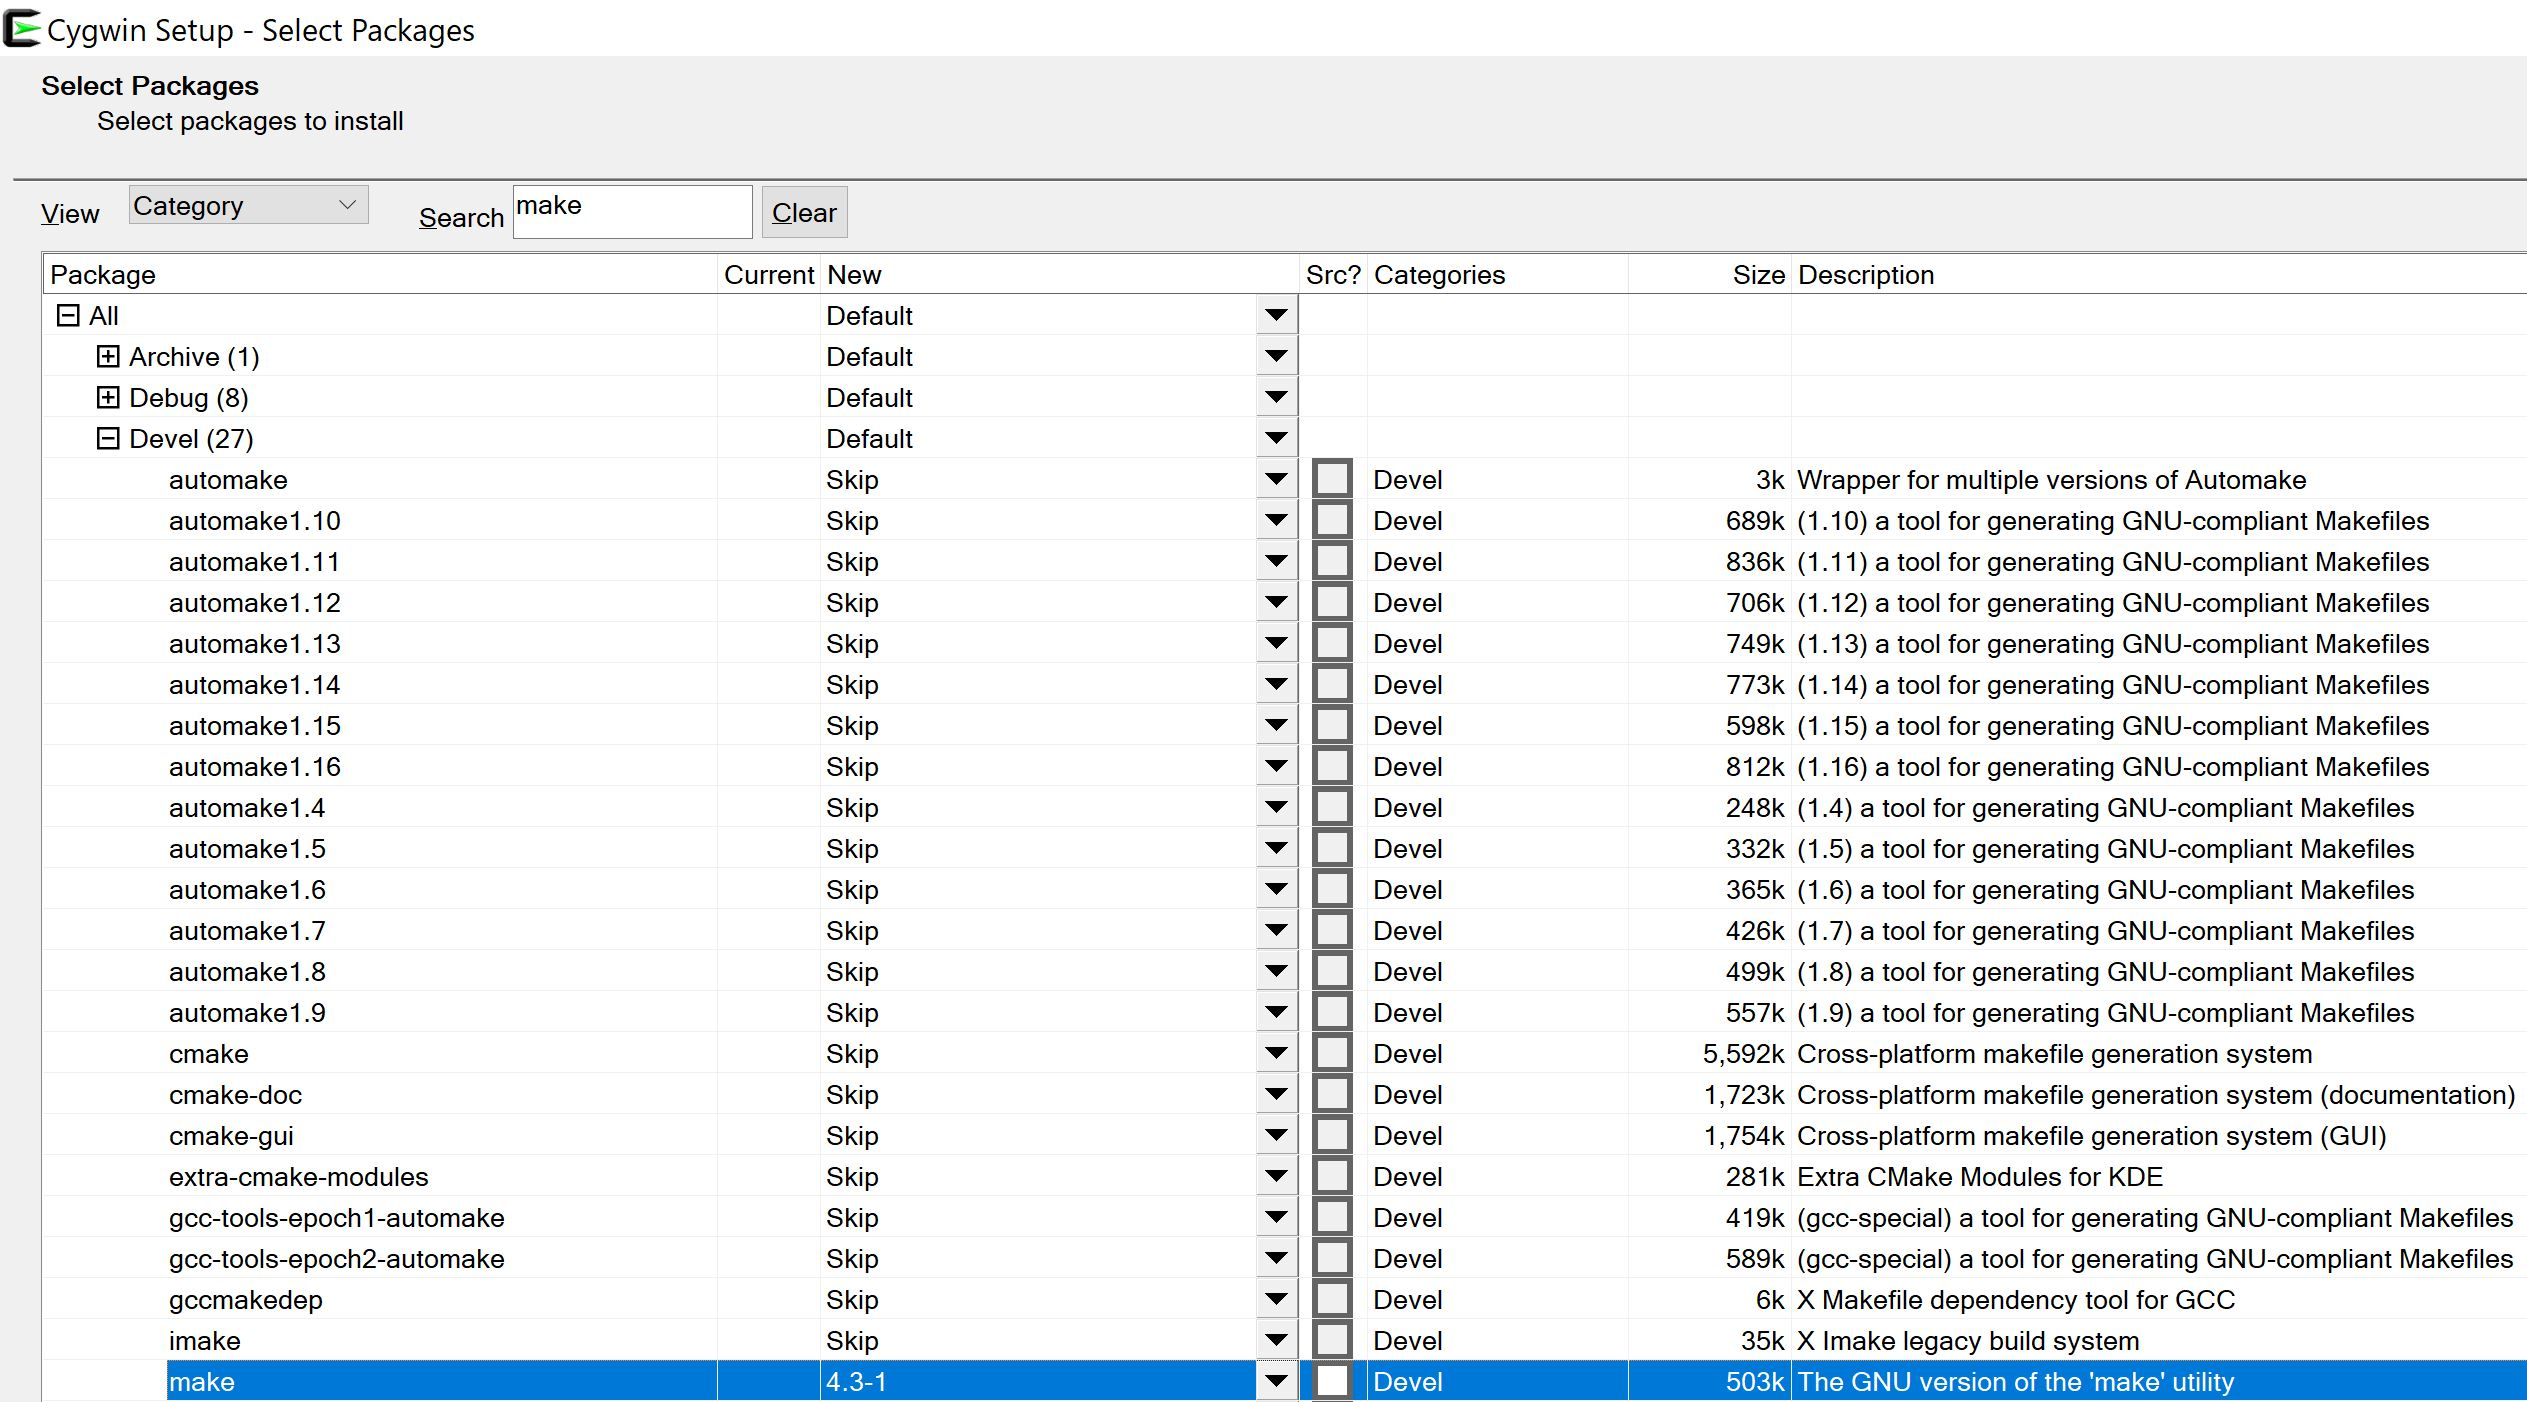
\includegraphics[scale=0.53]{figures/Capture.JPG}
    \caption{Eksempel på installasjon av pakken \texttt{make} i Cygwin.}
    \label{fig:Cygwin-setup}
\end{figure}

\subsection{Oppdatering av pakker etter installasjon}

Det er fort gjort å glemme å installere en pakke. Da kjører man simpelthen installasjonsprogrammet igjen. Like enkelt er det å oppgradere pakker. Installasjonsprogrammet holder styr på det man allerede har installert, og sammenlikner det med det som ligger på det distribujsonsstedet som man velger.
